\documentclass[11pt,letterpaper]{article}

\usepackage[T1]{fontenc}
\usepackage[spanish,es-nodecimaldot]{babel}
\usepackage[margin=2.5cm]{geometry}
\usepackage{amsmath,amssymb}
\usepackage{enumitem}
\usepackage{graphicx}
\usepackage[hidelinks]{hyperref}
\usepackage{multicol}
\emergencystretch=3em
\raggedbottom

\usepackage{csquotes}

\usepackage{caption}
\captionsetup{hypcap=false}

\usepackage{tikz}
\usetikzlibrary{positioning}
\usetikzlibrary{arrows.meta}

\usepackage[
    backend=biber,
    style=numeric,
    natbib=true
]{biblatex}

\addbibresource{bibliografia.bib}

% Bibliografía en bandera para evitar líneas sueltas (underfull) en columna angosta
\renewcommand*{\bibfont}{\normalfont\raggedright}

\title{
    Investigación N\textsuperscript{o} 1 RM3100 \\
    \large Información sobre el sensor y conceptos claves
}

\author{Yerko Jelcic Iturra}
\date{\today}

\begin{document}

\maketitle

\begin{abstract}
    El sensor RM3100 es un magnetómetro de tres ejes basado en tecnología magneto-inductiva (MI). A diferencia de los sensores de efecto Hall o magnetorresistivos (RM), no mide un voltage analógico proporcional al campo, sino que traduce el campo magnético a una frecuencia de oscilación que se cuantifica digitalmente. Esto otorga un ruido bajo (piso de ruido de $4pT/\sqrt{Hz}$ a $1Hz$), salida inherentemente digital sin acondicionamiento analógico, y ausencia de deriva de offset (bias drift) apreciable con la temperatura. El sistema completo consta de tres bobinas sensoras \textbf{(2 Sen-xy, 1 Sen-z)} y un ASIC controlador denominado \textbf{MagI2C}, que excita las bobinas y realiza el conteo temporal.
\end{abstract}

\begin{multicols*}{2}
\section{Principio físico}
El RM3100 pertence a la familia de sensores magneto-inductivos (MI). El cual, a diferencia de un fluxgate o un sensor de efecto Hall, no mide una tensión proporcional al campo, sino que traduce el campo externo en una variación de inductancia, y de ahí en una variación temporal que un contador digital puede leer directamente. 
El sensor es una bobina solenoidal de $N$ vueltas y longitud $l$, tal que se tiene $n = N/l$ vueltas por unidad de longitud, devanada sobre un núcleo de alta permeabilidad. Aplicando la ley de Ampere para la intensidad del campo $\vec{H}$, que solo depende de las corrientes de conducción, el campo que la propia bobina establece a lo largo del eje es $H_{bob} = \dfrac{N}{l}I = n I$. Por superposición con la componente axial del campo externo $\vec{H}_E$, el núcleo experimenta
\begin{equation}
    H = k_0I + H_E \qquad k_0\equiv n = \dfrac{N}{l}
    \label{eq:1}
\end{equation}
La constante $k_0$ es geométrica y no depende de la permeabilidad. Además, se trabaja en $H$, y no en $B$, para mantener esta parte de la cadena libre de la no linealidad del material \citep{leuzinger2010}.
Sin embargo, el comportamiento del núcleo se describe por su curva de magnetización $B(H)$, mostrada esquemáticamente en la Fig.~\ref{fig:curva-bh}. En un material ferromagnético blando, esta curva es no lineal, ya que para campos pequeños la respuesta es casi lineal (región de máxima pediente), luego aparece una curva y finalmente el material satura en $\pm B_s$, donde un incremento de $\vec{H}$ casi no afecta a $\vec{B}$.

De esto, conviene distinguir dos permeabilidades:
\begin{itemize}
    \item Permeabilidad de amplitud: $\mu = \dfrac{B}{H}$
    \item Permeabilidad incremental: $\mu_{inc} = \dfrac{dB}{dH}$
\end{itemize}

La primera corresponde a una relación estática entre B y H, ya que corresponde a la pendiente de la línea que va desde el origen hasta un cierto punto del ciclo de la histéresis para un valor dado de H. En cambio, la segunda representa la pendiente local de una cierta zona del bucle menor para un valor de intensidad de campo dado. A niveles bajos de excitación, la permeabilidad incvremental es igual a la permeabilidad inicial. Aumenta el valor de H hasta alcanzar un máximo y, a medida que el nivel de excitación aumenta, el núcleo se satura y la permeabilidad incremental se aproxima a la del vacio \citep{permeability}. Para las pequeñas oscilaciones de corriente que ocurren en el sensor alrededor de un punto de operación, la inductancia dependerá de $\mu_{inc}$ y no de $\mu$.

En la Fig.~\ref{fig:curva-bh}, $\mu_{inc}$ es máxima cerca del origen y disminuye hacia la saturación. En un núcleo balndo, la curva $B(H)$ es prácticamente \textit{anhisterética} (sin lazo de histéresis apreciable) y de simetría impar, $B(-H) = -B(H)$. Para el caso del sensor, el fabricante reporta la ausencia de la histéresis, que es la razón física por la que no presenta deriva de offset apreciable.

\begin{center}
    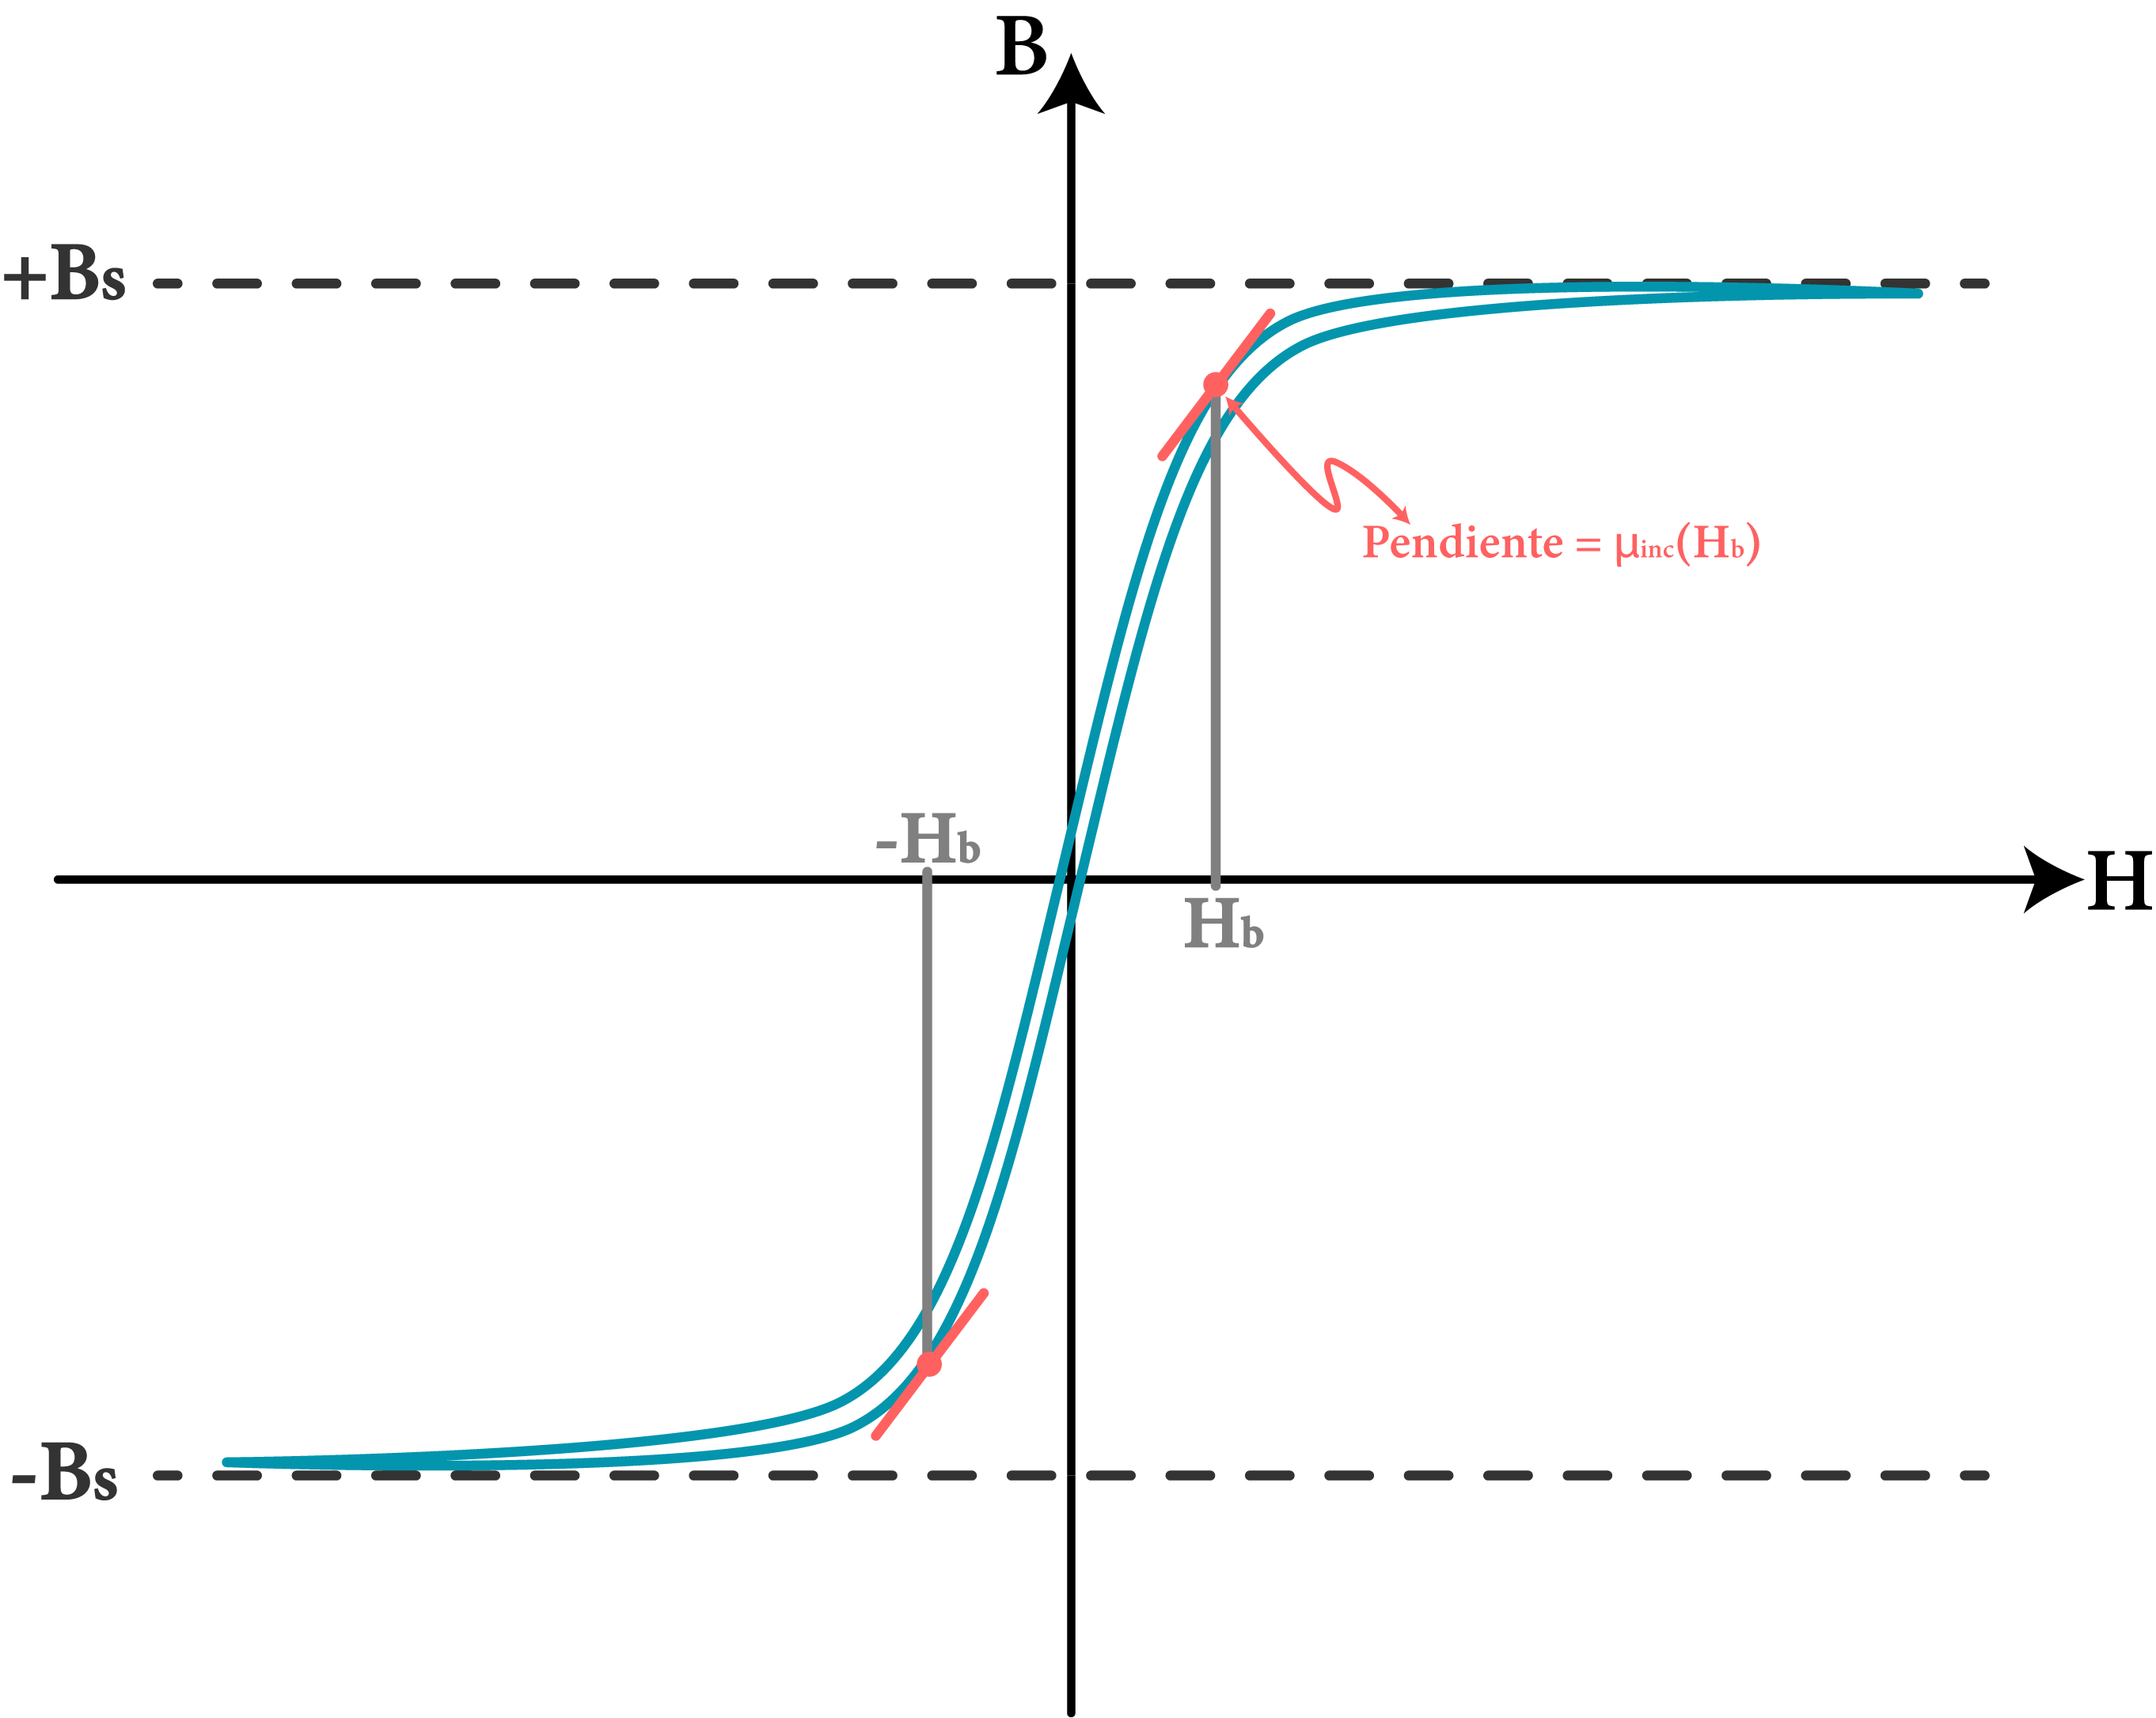
\includegraphics[width=0.8\columnwidth]{assets/curva_B-H.png}
    \captionof{figure}{Curva de magnetización B(H) de un núcleo ferromagnético blando. La permeabilidad incremental $\mu_{inc} = dB/dH$ es la pendiente local; en los puntos de operación $\pm H_b$ (región no lineal) la pendiente cambia con el campo, lo que da sensibilidad al sensor.}
    \label{fig:curva-bh}
\end{center}

Por otro lado, la inductancia se define como la relación entre el diferencial de flujo magnético $Nd\Phi = N\ A \ dB$ y la variación de corriente $I$, dónde $N$ corresponde al número de vueltas de la bobina, $B$ es la densidad del flujo magnético y $A$ es el área de la selección transversal. Además, usando la definición de la ecuación~\eqref{eq:1}, se obtiene que:
\begin{align}
    L = N\frac{d\Phi}{dI} &= NA\frac{dB}{dI} \notag \\[2pt]
  = NA\frac{dB}{dH}\frac{dH}{dI} &= NA\mu_{\mathrm{inc}}k_0 \notag \\[2pt]
  = \boxed{\frac{N^2A}{l}\mu_{\mathrm{inc}}(H)} &\equiv G\,\mu_{\mathrm{inc}}(H)
  \label{eq:2}
\end{align}

La inductancia es el factor geométrico G multiplicado por la permeabilidad incremental evaluada en el punto de operación. Por lo tanto, un cambio en el campo externo $H_E$ desplaza el punto de operación sobre la curva B-H (ecuación~\eqref{eq:1}), cambia la pendiente local $\mu_{inc}$ y, con ella, la inductancia (ecuación~\eqref{eq:2}). Esta cadena se resume en la Fig.~\ref{fig:efecto_campo_inductancia}.

\begin{center}
    
    \begin{tikzpicture}[
            block/.style={
                draw,
                rounded corners,
                align=center,
                minimum width=6cm,
                minimum height=1cm
            }
        ]

        \node[block, fill = blue!30] (campo) {Corriente de excitación $I$ \\y Campo externo $H_{\mathrm{ext}}$};
        
        \node[block, below = 0.8cm of campo] (campo total)
            {Campo total en el núcleo\\
            $H = k_0 I + H_E$};

        \node[block, below = 0.8cm of campo total] (punto)
            {Desplazamiento del punto de\\
            operación en la curva \textit{B-H}};

        \node[block, below = 0.8cm of punto] (permeabilidad)
            {Cambio en la $\mu_{\mathrm{inc}}$\\
            $\displaystyle \mu_{\mathrm{inc}}=dB/dH$};

        \node[block, below = 0.8cm of permeabilidad] (inductancia sensor)
            {Inductancia del sensor\\
            $L = G \mu_{inc}$};
        
        \node[block, below = 0.8cm of inductancia sensor] (relajacion)
            {Constante de relajación\\
            $\tau = L/R_b$};


        \node[block, below = 0.8cm of relajacion, fill = blue!30] (medicion)
            {Medida diferencial\\
            $\Delta t = t_+ - t_- \varpropto H_E$};

        \draw[-{Stealth}, thick] (campo) -- (campo total);
        \draw[-{Stealth}, thick] (campo total) -- (punto);
        \draw[-{Stealth}, thick] (punto) -- (permeabilidad);
        \draw[-{Stealth}, thick] (permeabilidad) -- (inductancia sensor);
        \draw[-{Stealth}, thick] (inductancia sensor) -- (relajacion);
        \draw[-{Stealth}, thick] (relajacion) -- (medicion);


    \end{tikzpicture}
    \captionof{figure}{Cadena Física de conversión del sensor magneto-inductivo. El campo externo modifica el punto de operación del núcleo, la permeabilidad incremental y la inductancia. Esto se ve reflejado en el oscilador de relajación, que traduce esa inductancia en tiempos, y la diferencia entre polaridad es proporcional a $H_E$.}
    \label{fig:efecto_campo_inductancia}
\end{center}

\subsection{Oscilador L/R}
El sensor consiste en una conexión en serie con un resistor de bias (polarización de un campo magnético de referencia, conocido y controlado, que el circuito aplica deliberadamente al núcleo para fijar su punto de operación en un lugar elegido de la curva B-H) $R_b$. Ocupando la ley de Kirchhoff, se obtiene de la Figura \ref{fig:circuito-RL}, la siguiente ecuación diferencial del circuito

\begin{align}
    V_S &= V_L + V_R \notag \\
    &= L\dfrac{dI}{dt} + R_b I
\end{align}

donde $V_S$ es el voltaje del Schmitt Trigger. Resolviendo esto, se obtiene que:

\begin{align}
    \dfrac{dI}{dt}
        &= \dfrac{V_S - R_b I}{L} \notag\\
        &= -\dfrac{R_b}{L}\left(I - \dfrac{V_S}{R_b}\right) \notag\\
        &= -\dfrac{R_b}{L}\left(I - I_{\infty}\right) \notag\\
    \intertext{El equilibrio ($dI/dt = 0$) define $I_{\infty} = V_S/R_b$. Con $x = I - I_{\infty}$ (luego $dx = dI$):}
    \dfrac{dx}{dt}
        &= -\dfrac{R_b}{L}\,x \notag\\
    \dfrac{dx}{x}
        &= -\dfrac{R_b}{L}\,dt \quad \Big/\!\int \notag\\
    \ln(x)
        &= -\dfrac{t}{\tau} + \ln(C), \quad \tau = \dfrac{L}{R_b} \notag\\
    \Longrightarrow\ x
        &= C\,e^{-t/\tau} \notag\\
    \intertext{Deshaciendo el cambio y aplicando $I(0) = I_0$:}
    I - I_{\infty}
        &= C\,e^{-t/\tau} \notag\\
    I(t)
        &= I_{\infty} + C\,e^{-t/\tau} \notag\\
    I_0
        &= I_{\infty} + C
         \ \Longrightarrow\ C = I_0 - I_{\infty} \notag\\
    \Longrightarrow
        &\  \boxed{I(t) = \,I_{\infty} + (I_0 - I_{\infty})\,e^{-t/\tau}\,}
    \label{eq:3}
\end{align}
de la eq. \ref{eq:3} apare la constante de tiempo de relajacióm $\tau = L / R_b$. Como $L=L(H)$ por la \ref{eq:2}, entonces $\tau = \tau(H)$, es decir, medir el tiempo de relajación es medir, en cierta relación, la inductancia, y por lo tanto, el campo.

\begin{center}
    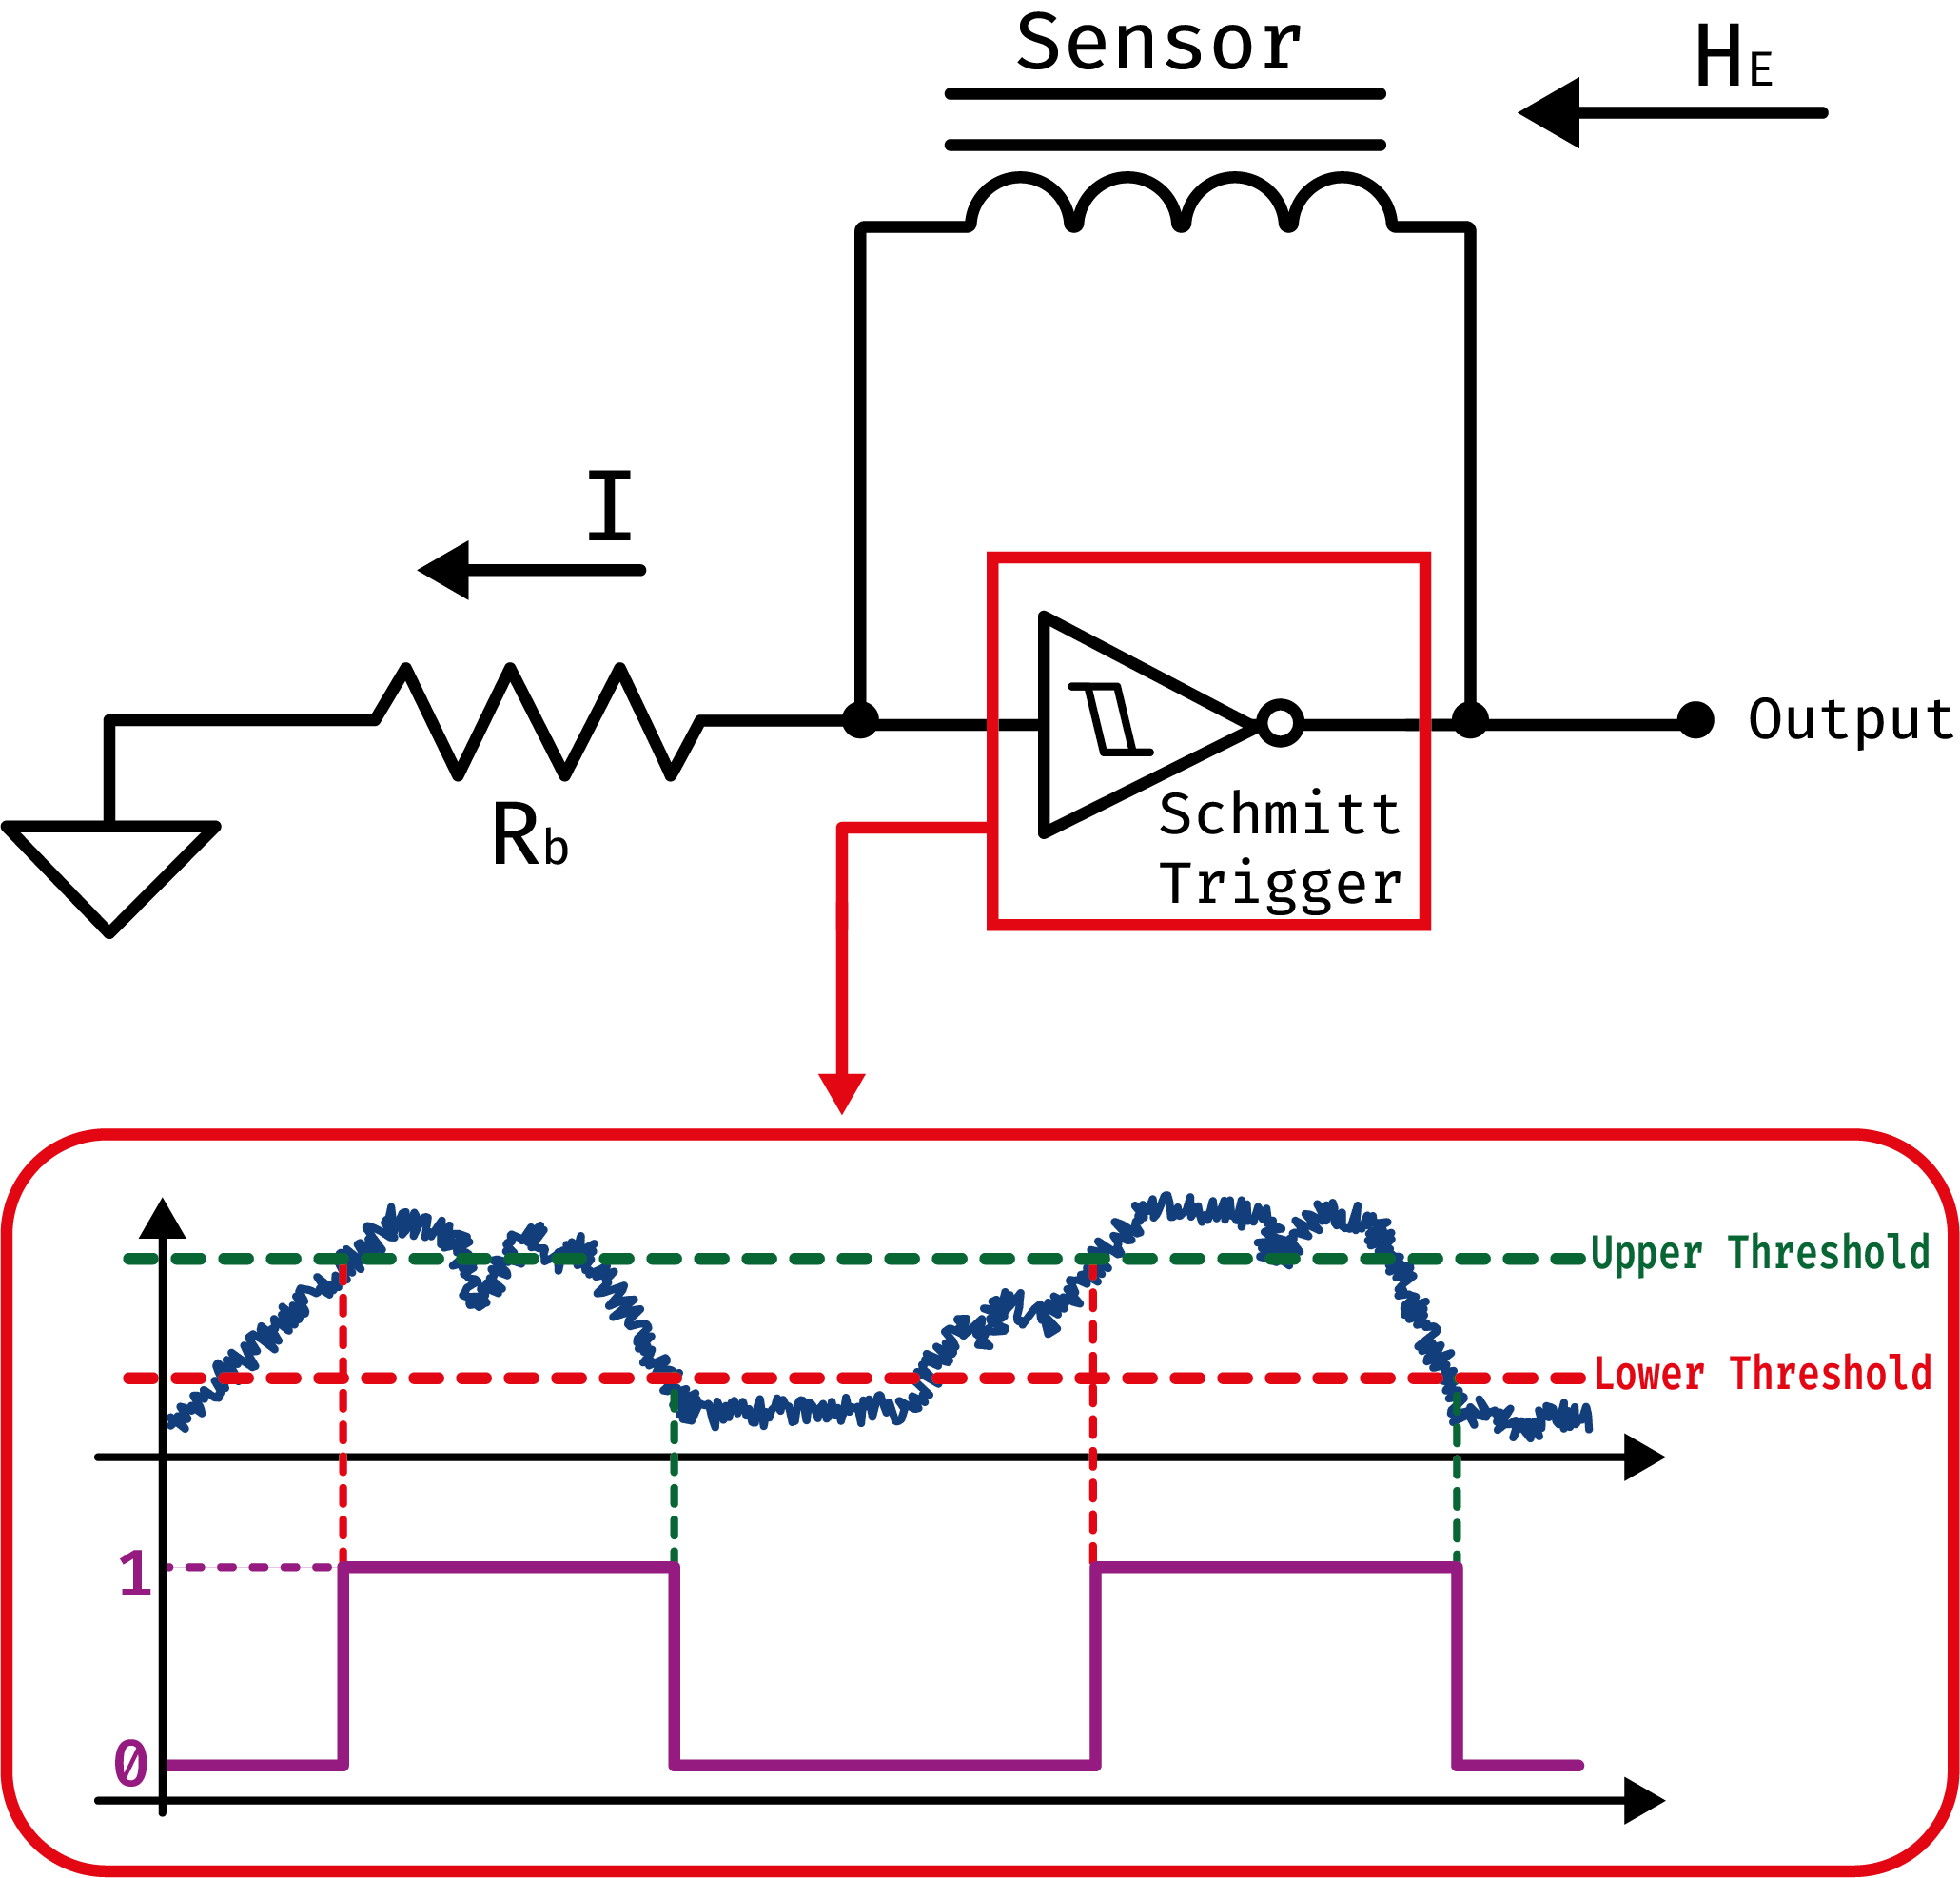
\includegraphics[width=0.8\columnwidth]{assets/Circuit R-L.png}
    \captionof{figure}{En la parte superior de la Figura se presenta el Basic MI Sensing Circuit \citep{leuzinger2010}, compuesto por el sensor inductivo $L$, el inversor Schmitt Trigger y la resistencia $R_B$. El recuadro inferior muestra la relación temporal entre la señal de entrada analógica y la salida digital resultante, donde el trazo azul representa la variación de voltaje en el nodo de entrada del Schmitt Trigger, la línea verde corresponde al umbral superior (Upper Threshold) y la línea roja al umbral inferior (Lower Threshold).}
    \label{fig:circuito-RL}
\end{center}

Añadido a esto, el Schmitt trigger de la Fig. \ref{fig:circuito-RL}, que corresponde a un tipo de entrada lógica que proporciona histéresis o dos niveles de voltaje de threshold diferentes para el edge ascendente y descendente. Es decir, sensa una tensión proporcional a la corriente y conmuta su salida cuando esa tensión cruza un umbral. Para entender mejor esto, se tomará un semiciclo de carga que lleva corriente desde $-I_{th}$ hasta $I_{th}$, con umbrales simétricos $I_{th} = V_{th}/R_b$, por lo que imponiendo estas condiciones en la eq. \ref{eq:3}:
\begin{equation*}
    I_{th} = I_{\infty} + (-I_{th}-I_{\infty})e^{-T/\tau}
\end{equation*}
despejando la exponencial:
\begin{align}
    &e^{-T/\tau}
        = \dfrac{I_{\infty} - I_{th}}{I_{\infty} + I_{th}} \notag \\
    &\Longleftrightarrow\ T
        = \tau \ln\!\left(\dfrac{I_{\infty} + I_{th}}{I_{\infty} - I_{th}}\right) \notag \\
    &\boxed{\;T = \dfrac{L}{R_b}\,
        \ln\!\left(\dfrac{V_S + V_{th}}{V_S - V_{th}}\right)
        }= K\,\dfrac{L}{R_b}\;
    \label{eq:4}
\end{align}

El resultado obtenido en la eq. \ref{eq:4} es que el tiempo de un semiciclo es proporcional a $L$ (y por lo tanto a $\mu(H)$), con un factor $K$ que depende unicamente de la excitación de $V_S$ y de los umbrales $V_{th}$. La condición de oscilacion es $V_S > V_{th}$, para que el argumento del logaritmo sea positivo y finito.


\section{Arquitectura del sensor}

\section{Modelo de medición}

\section{Modelo de operación}

\section{Interfaces y mapa de registros}

\section{Especificaciones de desempeño}

\section{Consideraciones prácticas}
\section{Conceptos}
\begin{itemize}
    \item \textbf{Magneto-Inductivo (MI)}: El sensor es un inductor cuya L depende del campo.
    \item \textbf{ASIC}: Circuito integrado para aplicaciones especificas.
    \item \textbf{Oscilador L/R}: El campo se traduce a periodo de oscilación (dominio de frecuencia).
    \item \textbf{Cycle count}: Parámetro que fija el compromiso entre ruido, resolución, velocidad y consumo.
    \item \textbf{Ganancia (LSB/$\mu$T)}: Factor de conversión, dependiente del cycle count. Además es la base de la conversión a $\mu$T.
    \item \textbf{MagI2C}: ASIC que excita, cuenta y expone registros. Es el punto de integración con el microcontrolador.
    \item \textbf{POLL vs CMM}: Medición bajo demanda frente a medición continua periódica.
    \item \textbf{TMRC y limite por cycle count}: La tasa efectiva es el mínimo entre lo pedido por TMRC (Configuración de la Tasa con el Registro).
    \item \textbf{DRDY/STATUS}: Mecanismo de sincronización de datos listo.
    \item \textbf{Formato 24 bits con signo}: Cada eje son 3 bits en complemento a dos.
    \item \textbf{Calibración hard/soft-iron}: Impresindible para medición absoluta o compassing.
\end{itemize}



\printbibliography
\end{multicols*}

\end{document}